\subsection*{Task 4}

\subsubsection*{a)}

\begin{figure}[h!]
  \centering
  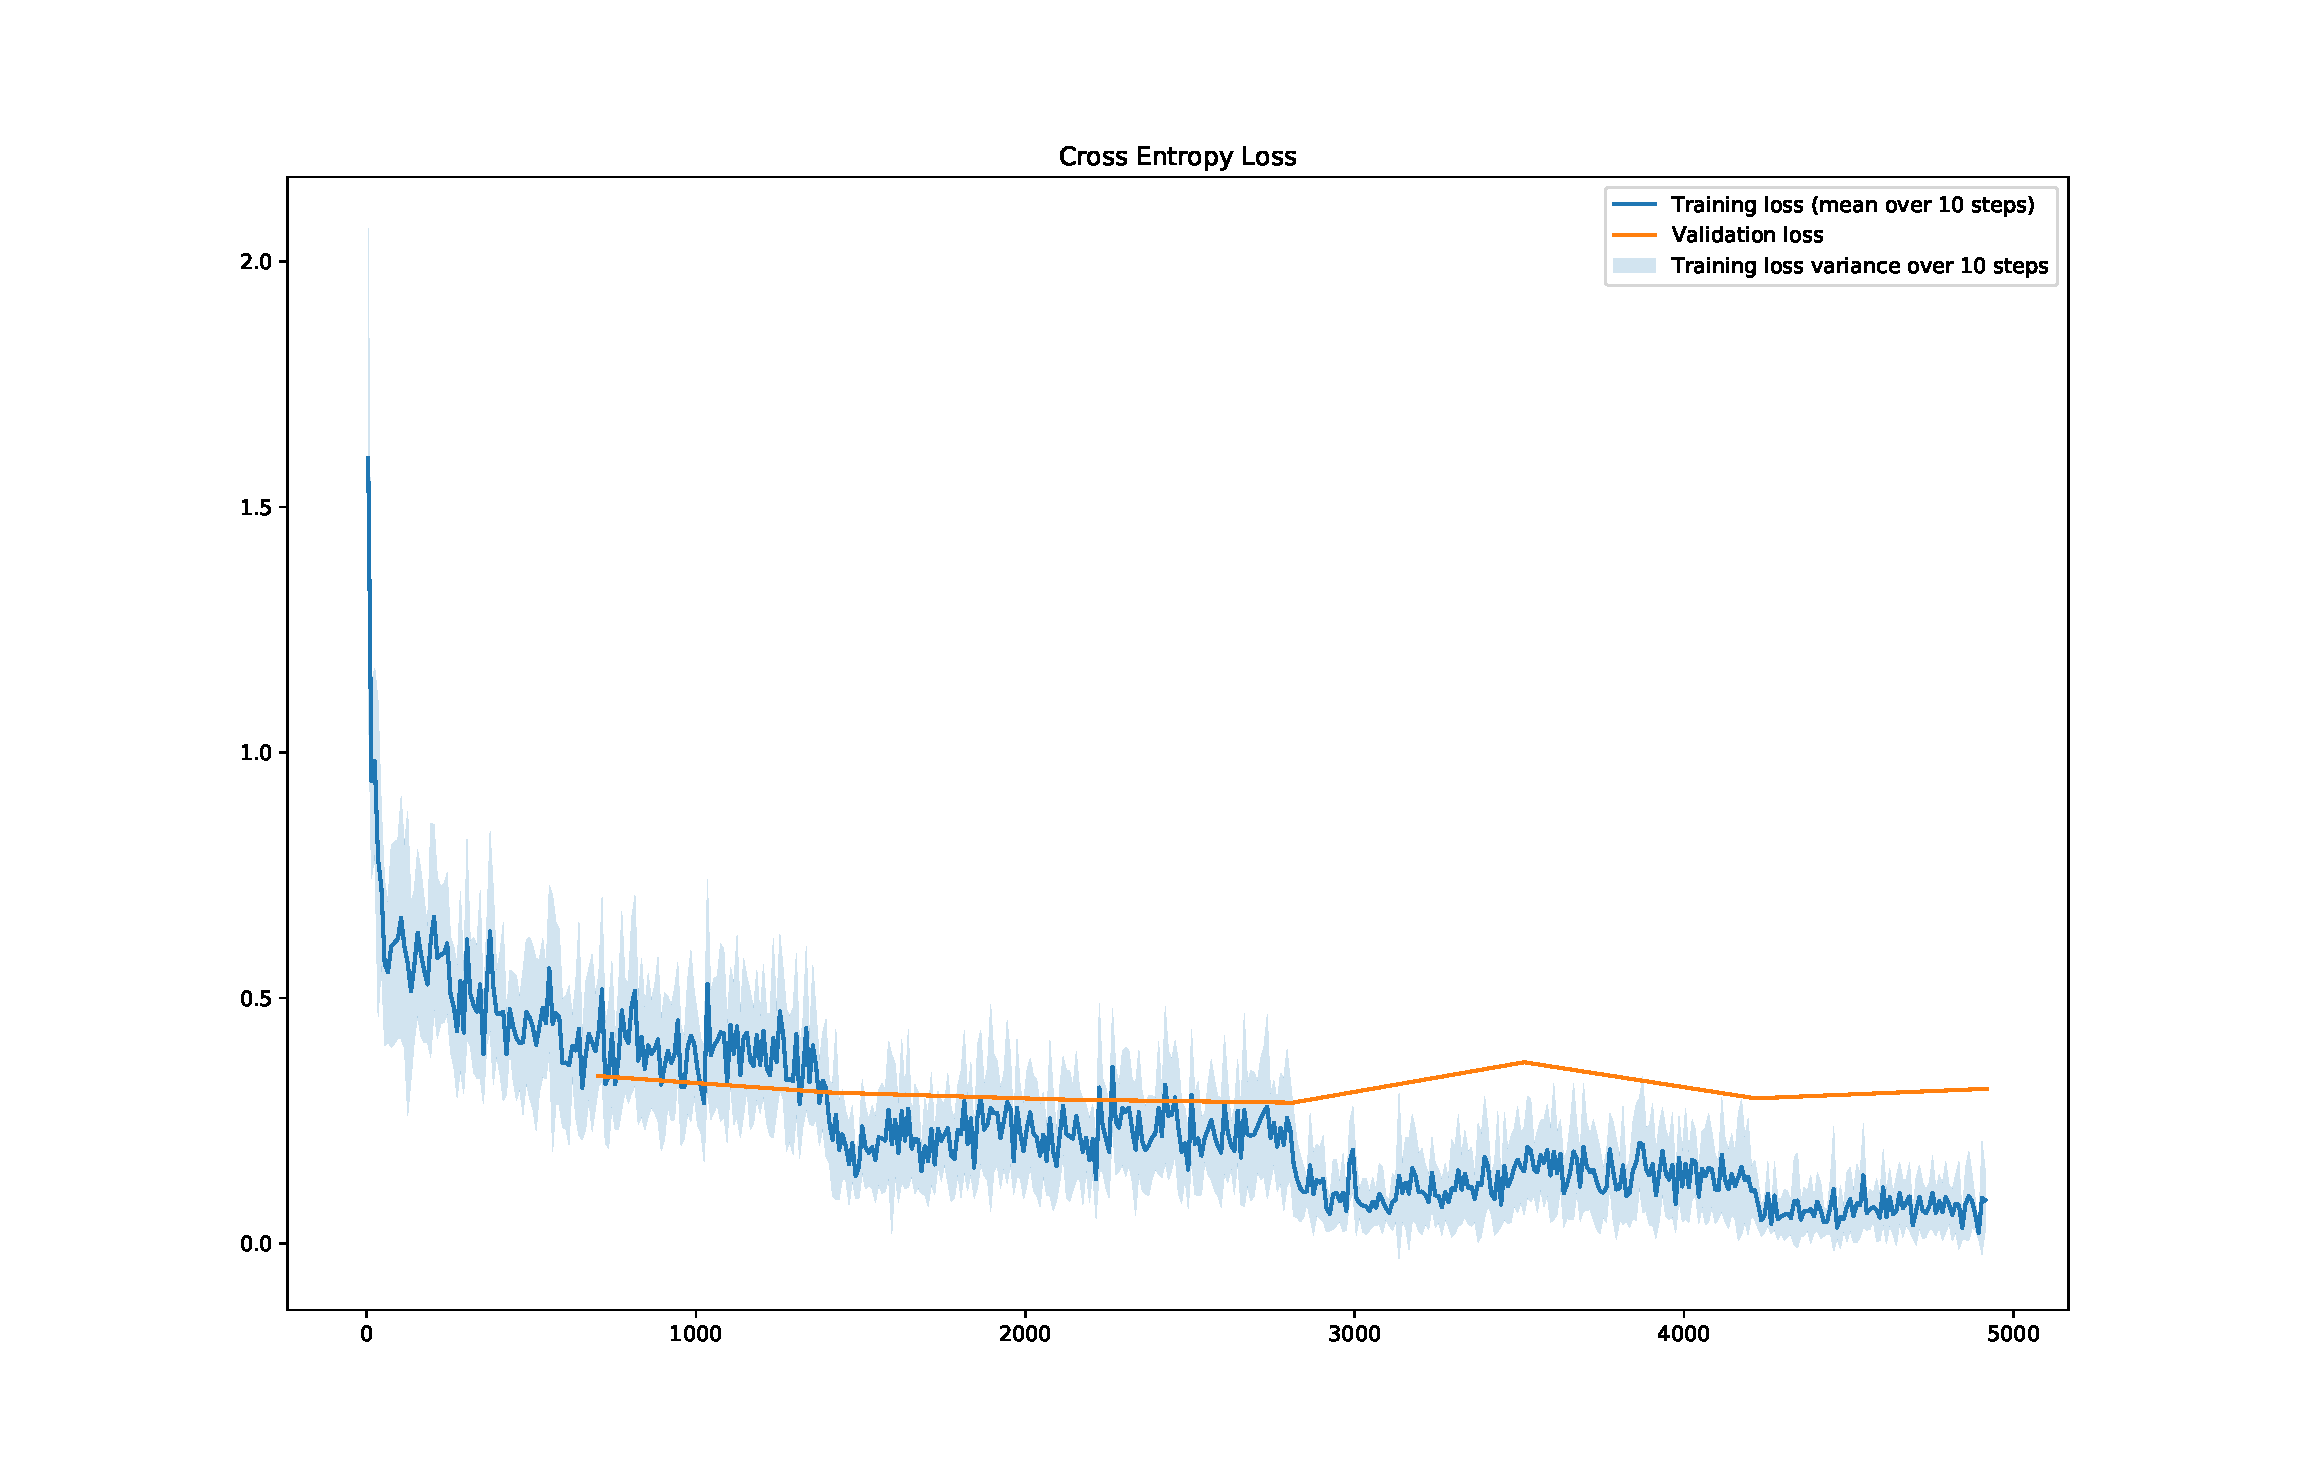
\includegraphics[clip,trim=0cm 2cm 0cm 2cm, width=\textwidth]{figures/Task4a.pdf}
  \caption{Training and validation loss over training.}
  \label{fig:task4:a}
\end{figure}

Results from transfer learning with Resnet18 for the CIFAR-10 dataset is shown in \cref{fig:task4:a}, with Adam optimizer, batch size of 32 and learning rate of $5\cdot10^{-5}$. Images in the dataset are resized to $224\times224$, and normalized with \texttt{mean:}$(0.485,0.456,0.406)$ and \texttt{std:}$(0.229,0.224,0.225)$. The final test accuracy with these parameters is 0.8727.


\subsubsection*{b)}

From \cref{fig:task4:b}, we see that each filter specializes in some feature of the original image. We see that e.g filter 14 activates on vertical lines and filter 26 activates on horizontal lines, and from the corresponding weights we see that both activate at the center of the image.

\begin{figure}[h!]
  \centering
  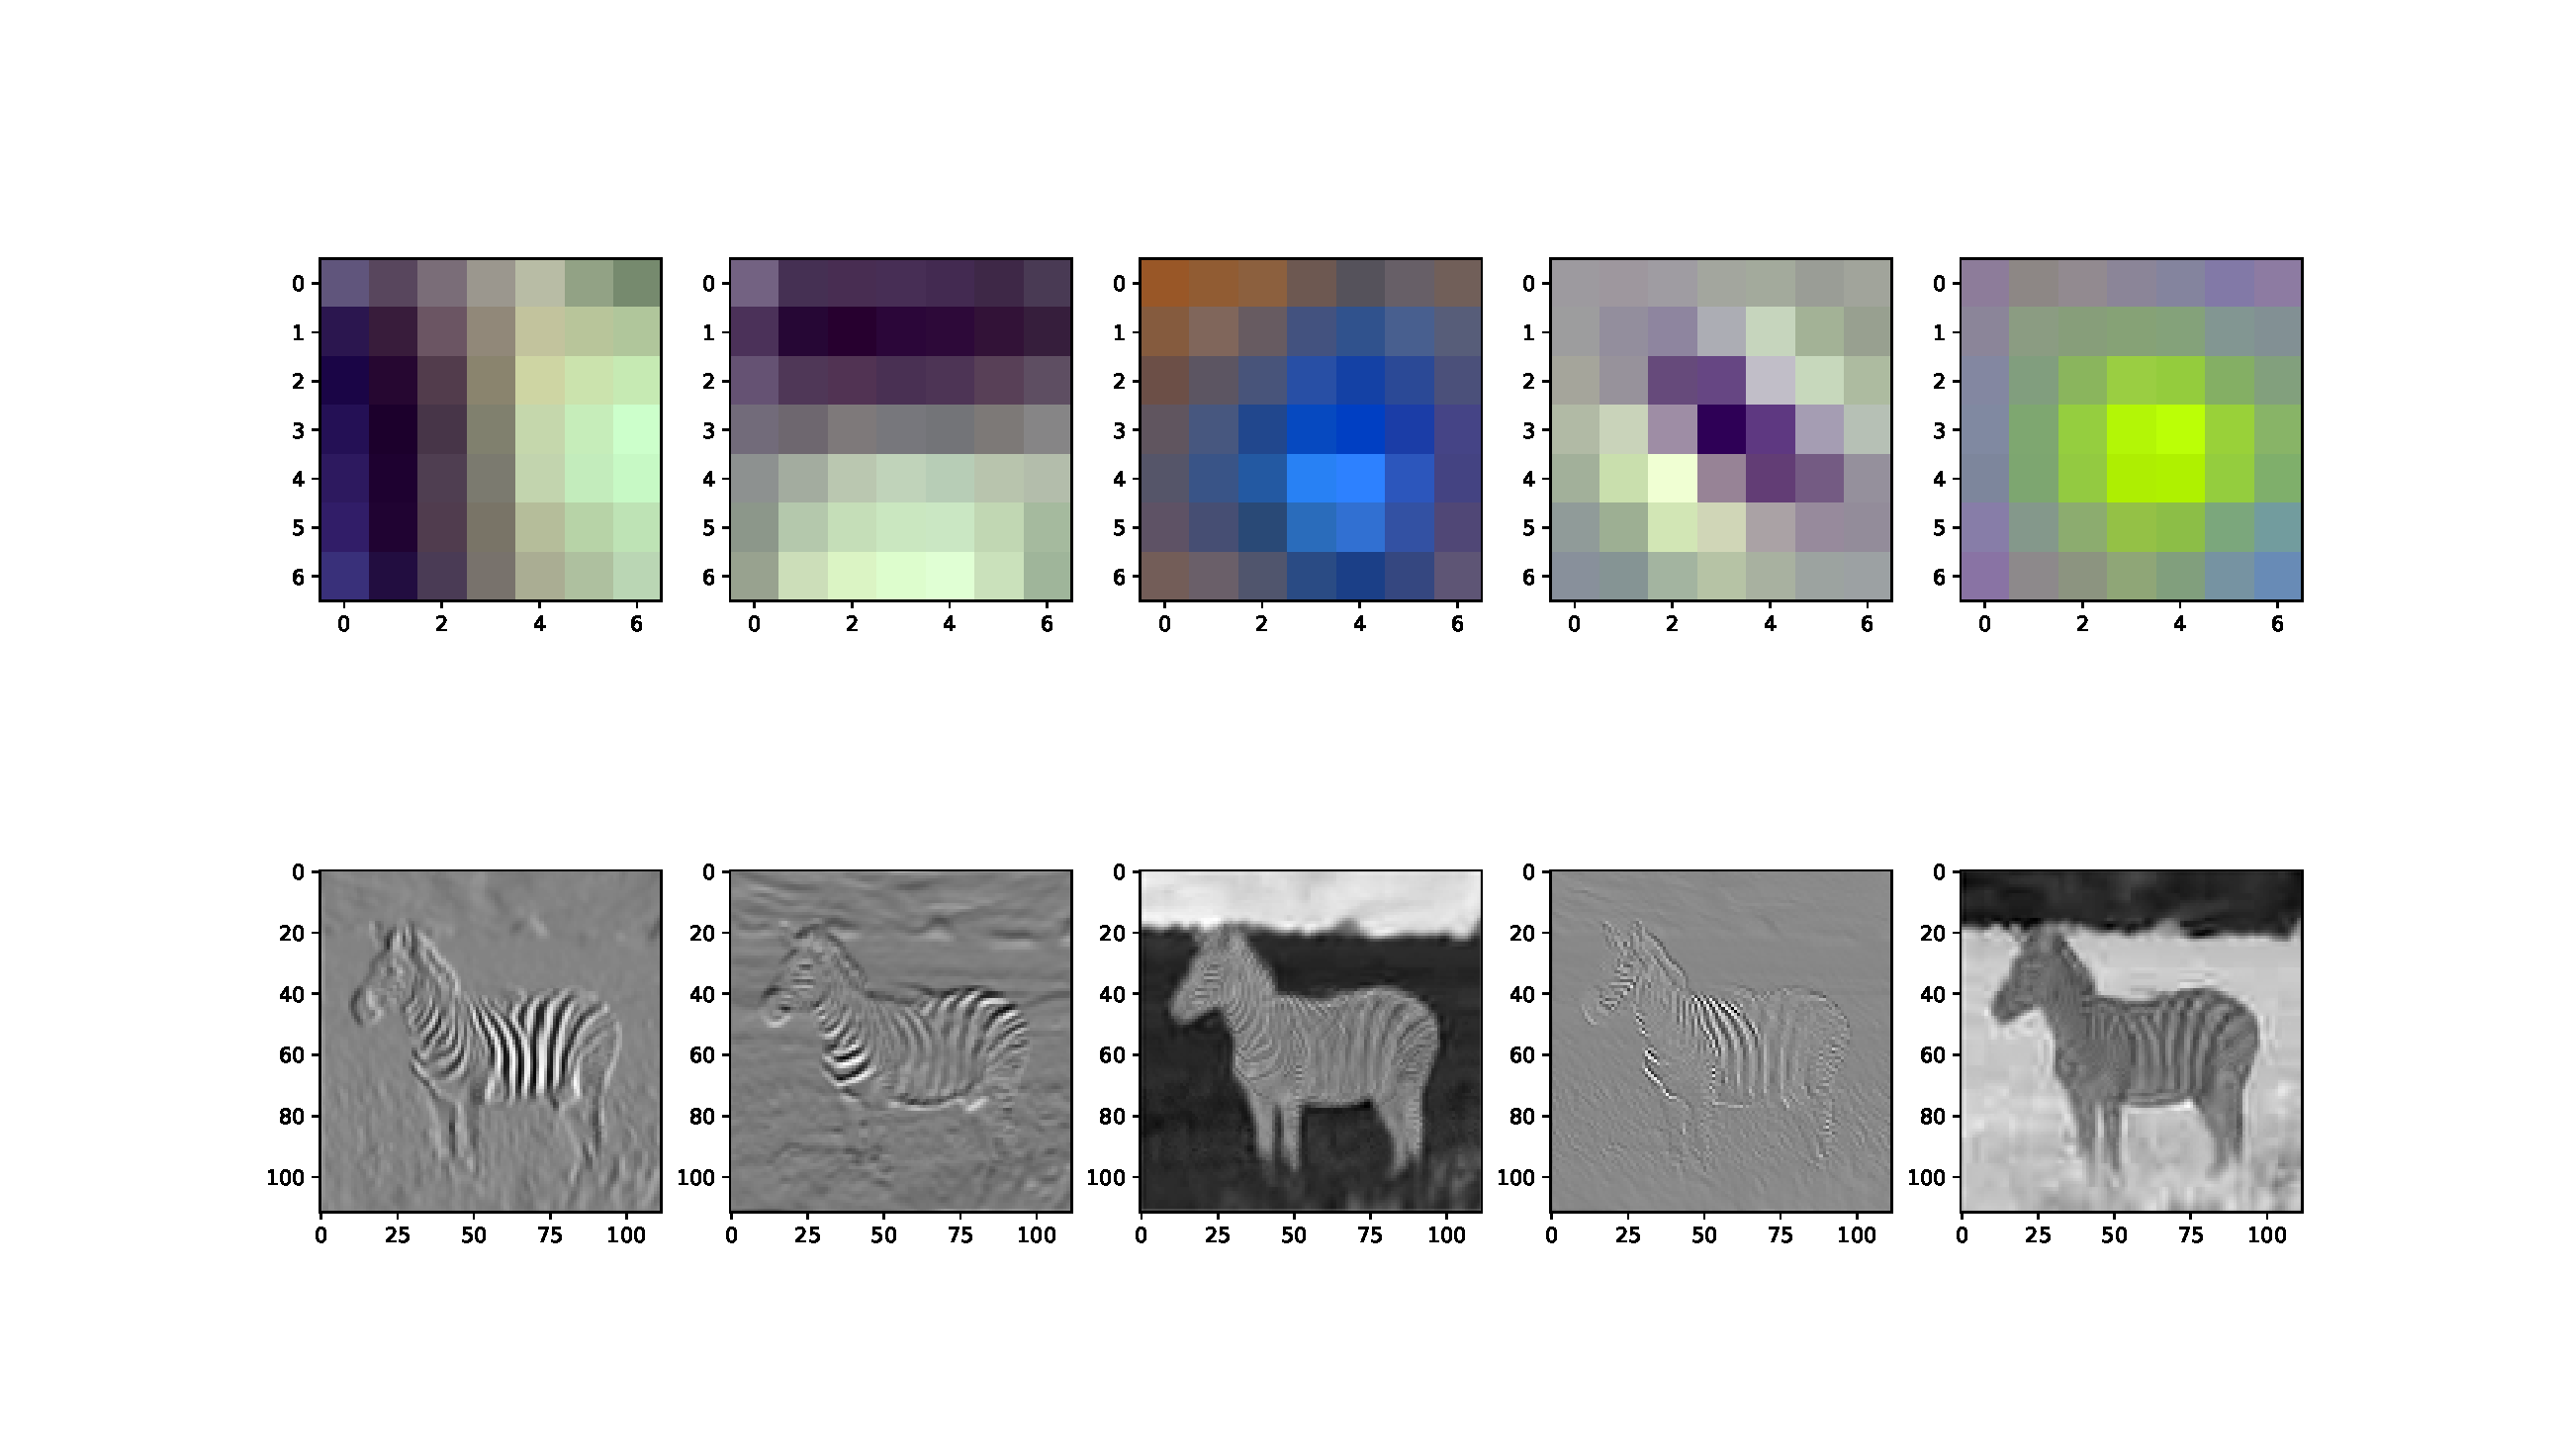
\includegraphics[clip,trim=4cm 2cm 4cm 2cm, width=\textwidth]{figures/Task4b.pdf}
  \caption{Filter weights (top row) and activation of corresponding filter (bottom row) of the first convolutional layer in ResNet18, with filter indices [14,26,32,49,52].}
  \label{fig:task4:b}
\end{figure}



\subsubsection*{c)}

The activations of the ten first filters from the last convolutional layer is shown in \cref{fig:task4:c}, which now are more abstract compared to the output of the first layer in \cref{fig:task4:b}. It is difficult to interpret these activations in any intuitive way, but this is what the network ultimately looks for in a zebra before making the classification.

\begin{figure}[h!]
  \centering
  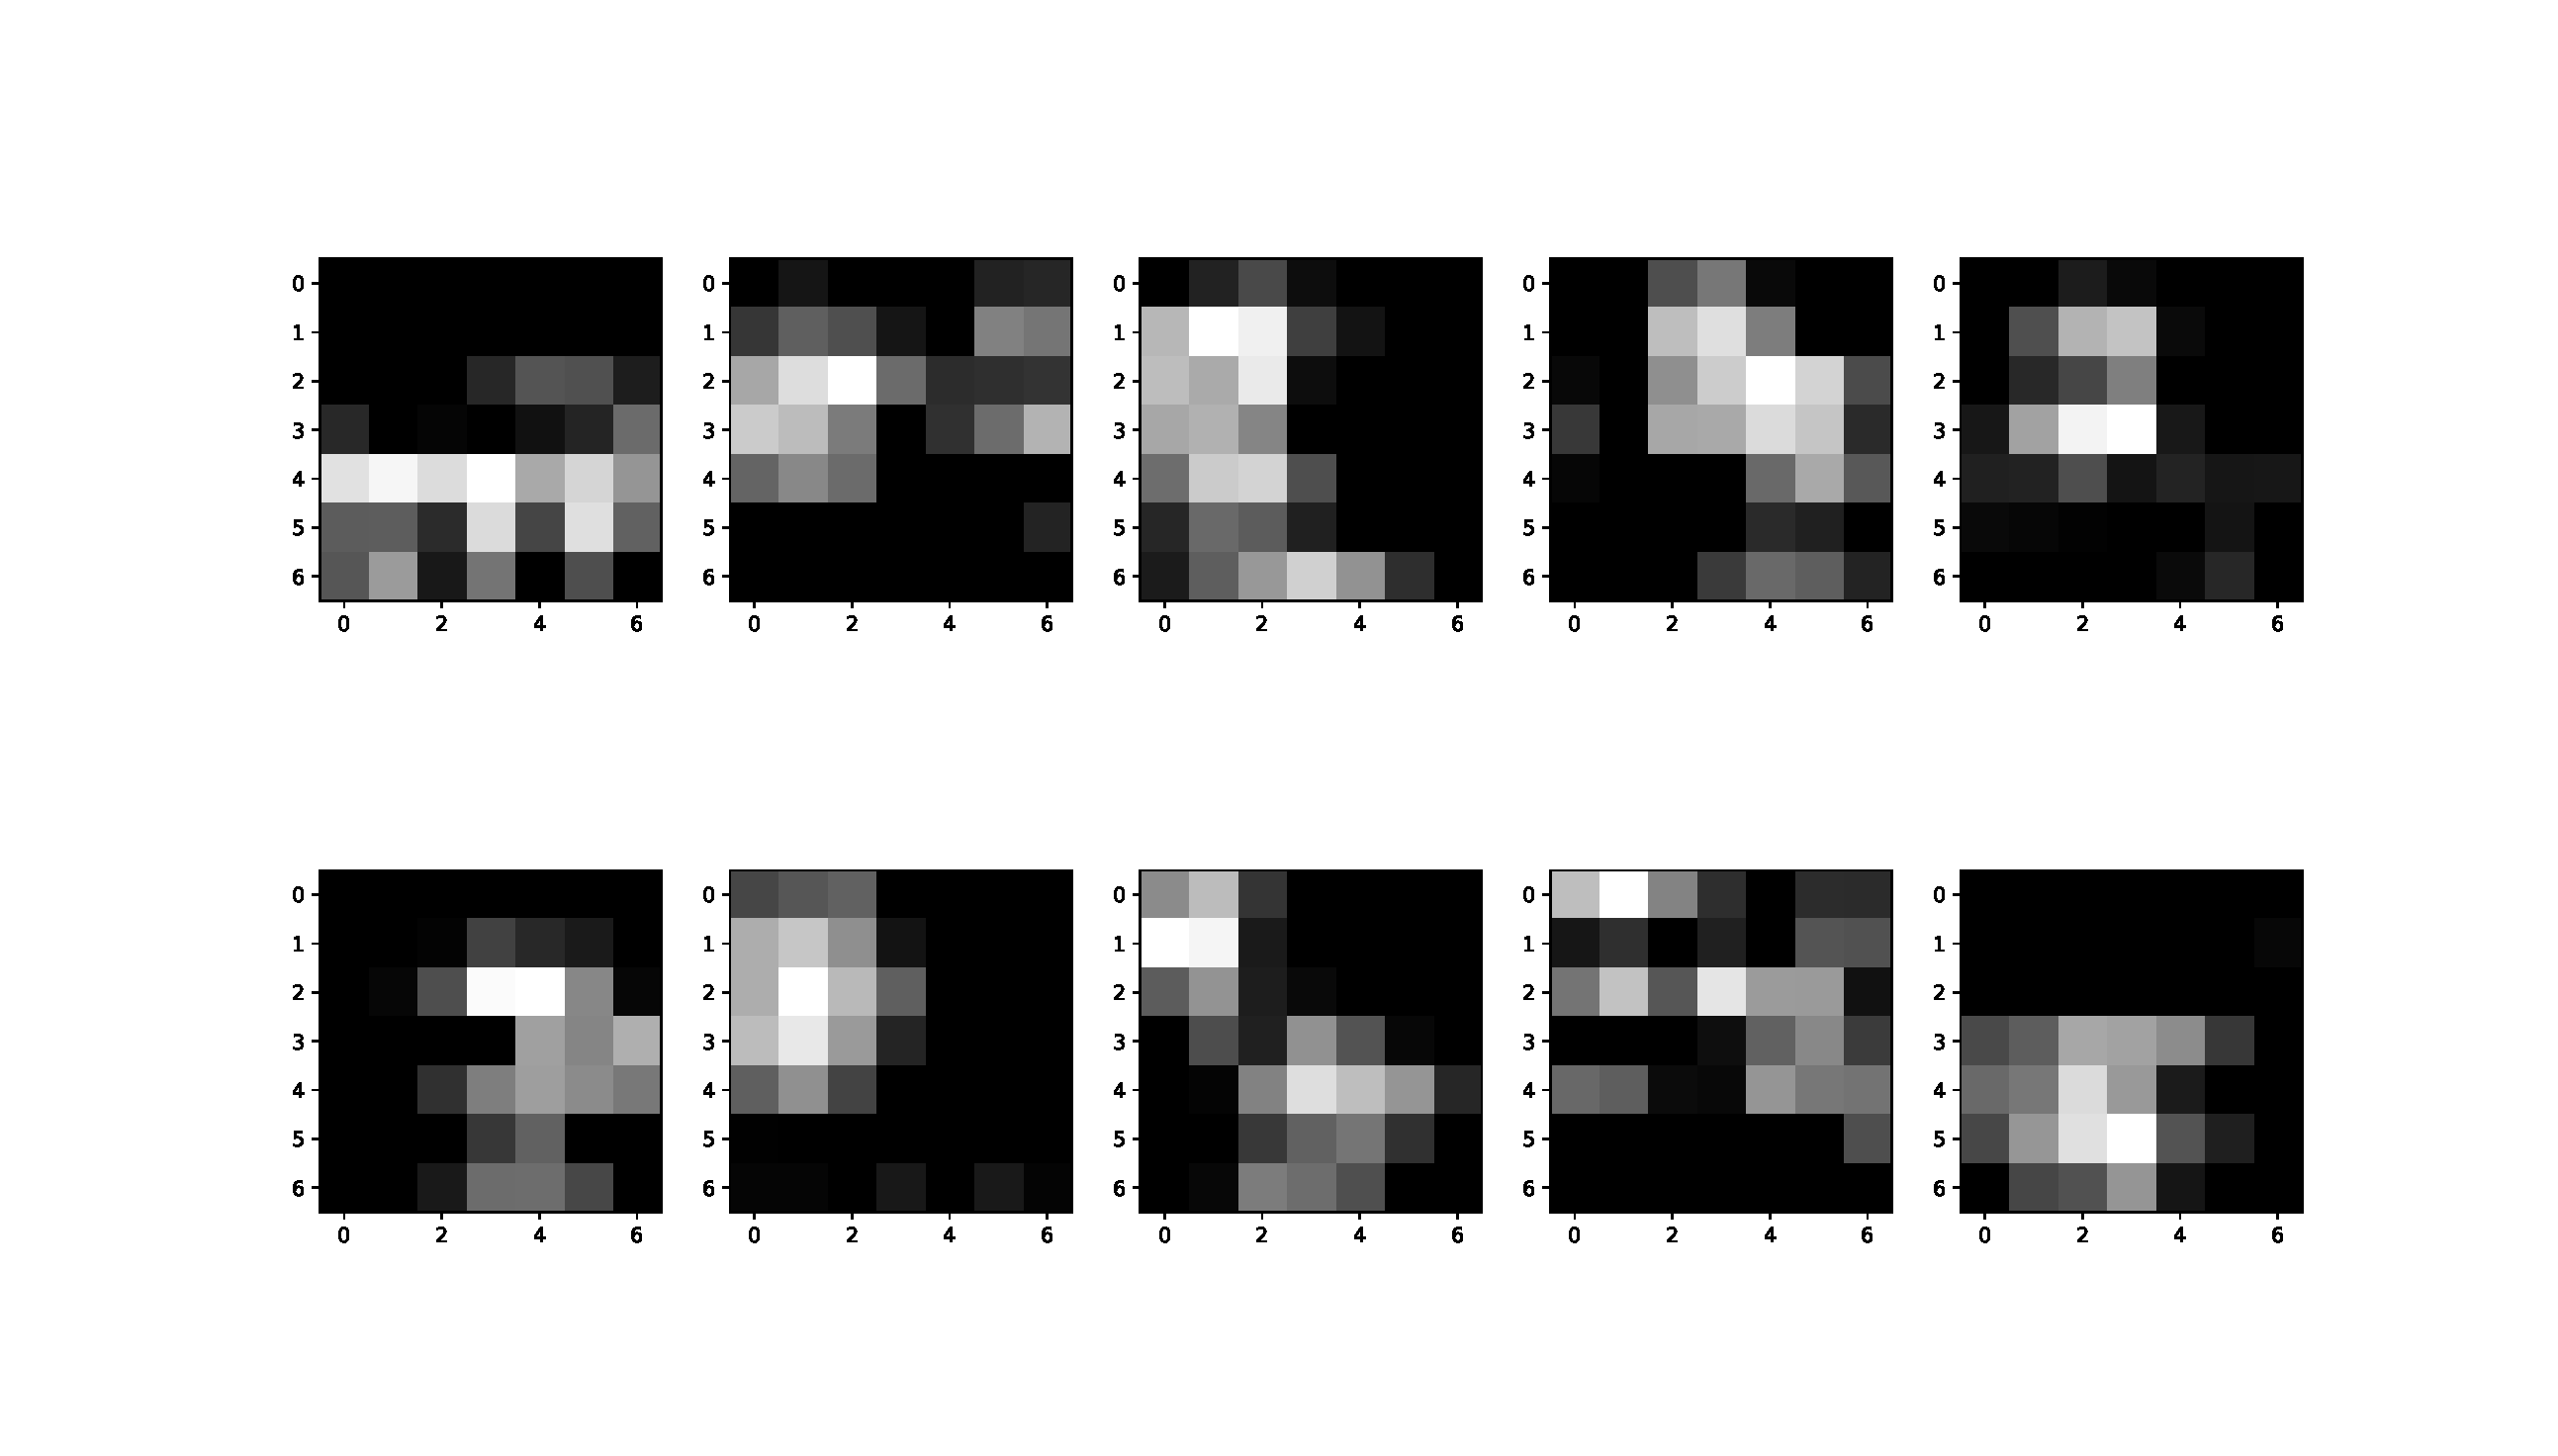
\includegraphics[clip,trim=4cm 2cm 4cm 2cm, width=\textwidth]{figures/Task4c.pdf}
  \caption{Activation of last convolutional layer in ResNet18, with filter indices 0-9, left to right, top to bottom.}
  \label{fig:task4:c}
\end{figure}


